\appendix
\chapter*{LAMPIRAN}
\addcontentsline{toc}{chapter}{LAMPIRAN}
\setcounter{section}{0} % Mengatur ulang penomoran section
\setcounter{page}{1}

\renewcommand{\thesection}{\Alph{section}}
\renewcommand{\thesubsection}{\Alph{section}.\arabic{subsection}\hspace{-0.25cm}}
\renewcommand{\thepage}{L - \arabic{page}}


\numberwithin{figure}{section}
\section{Data Diri {\penulisPertama}}

\begin{itemize}
	
	\item Riwayat Diri \\
	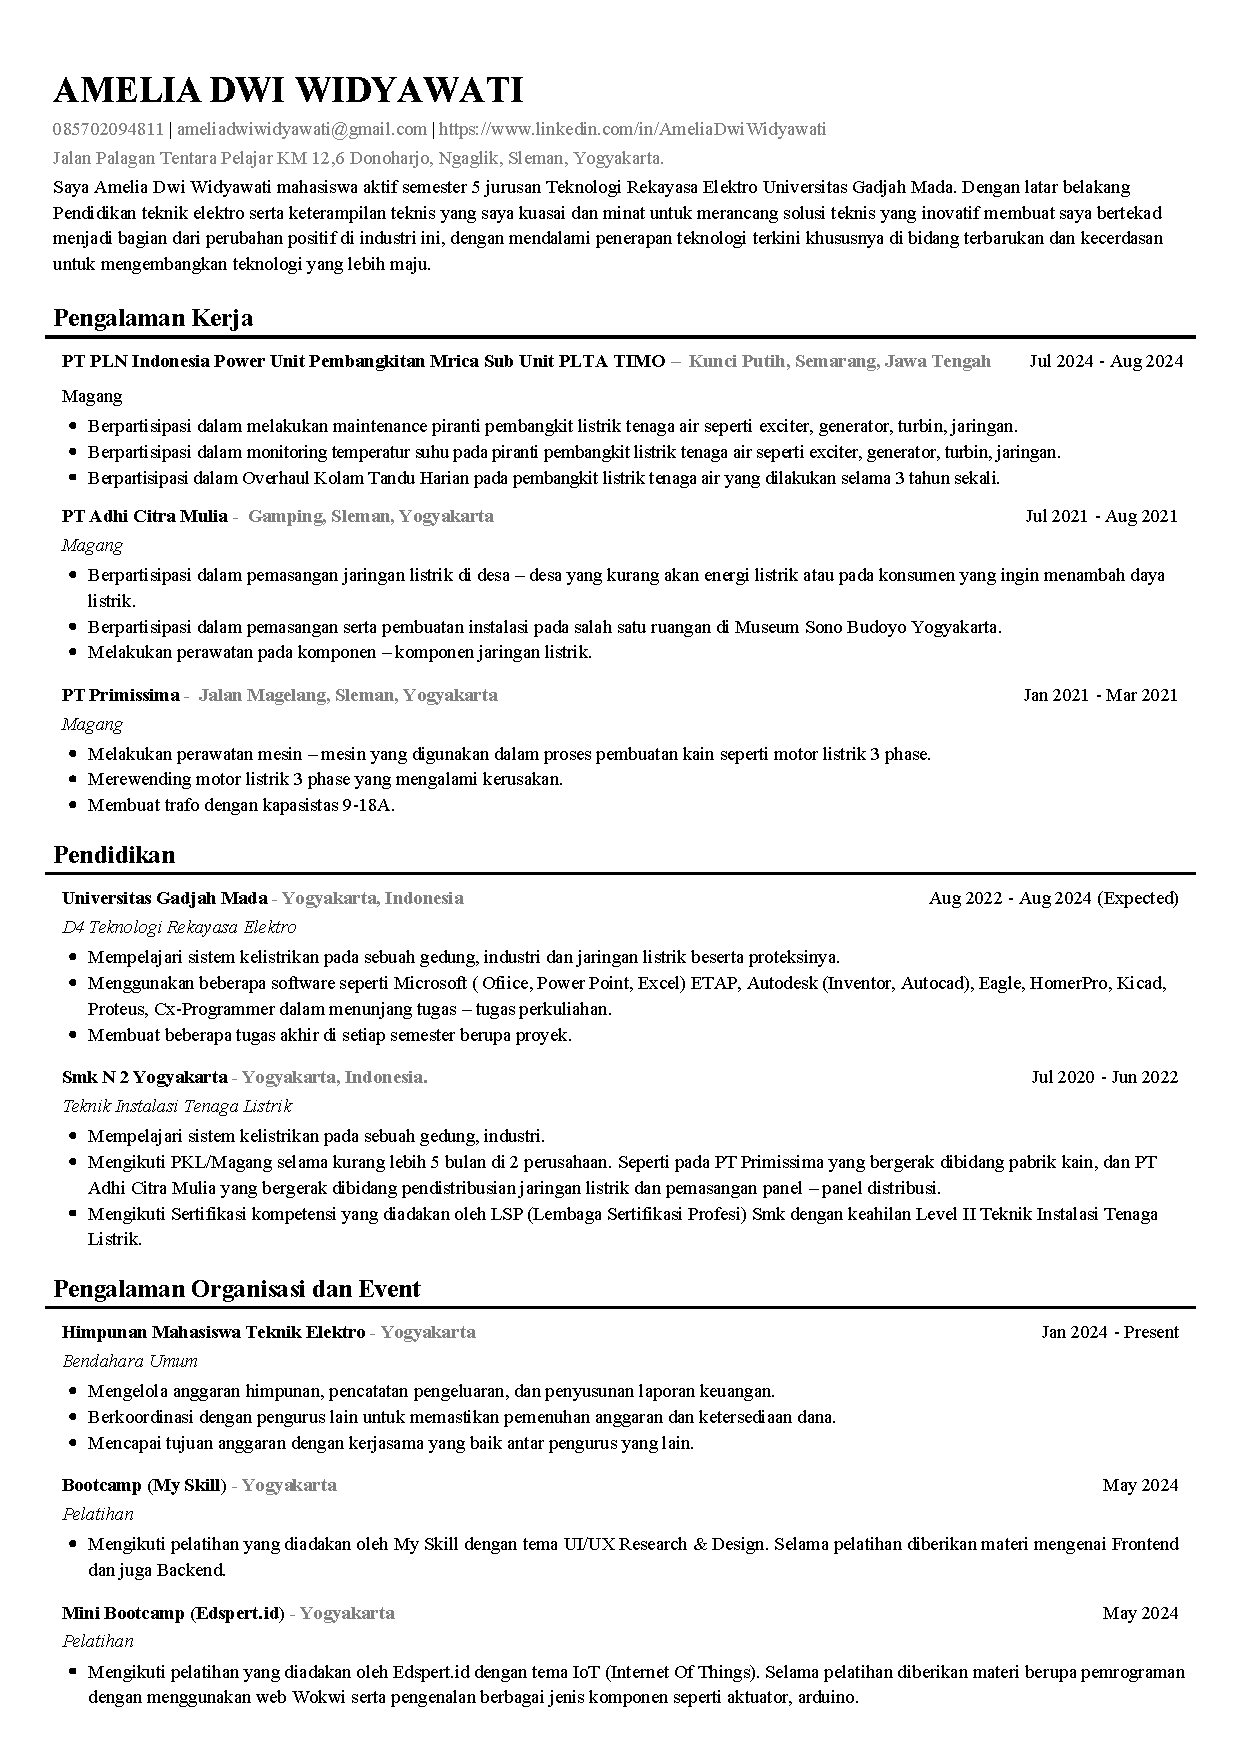
\includegraphics[scale=0.69,page=1]{dokumen/cv_amelia.pdf}
	\newpage
	\includegraphics[scale=0.69,page=2]{dokumen/cv_amelia.pdf}
	
	\newpage		
	\item Transkrip Nilai\\
	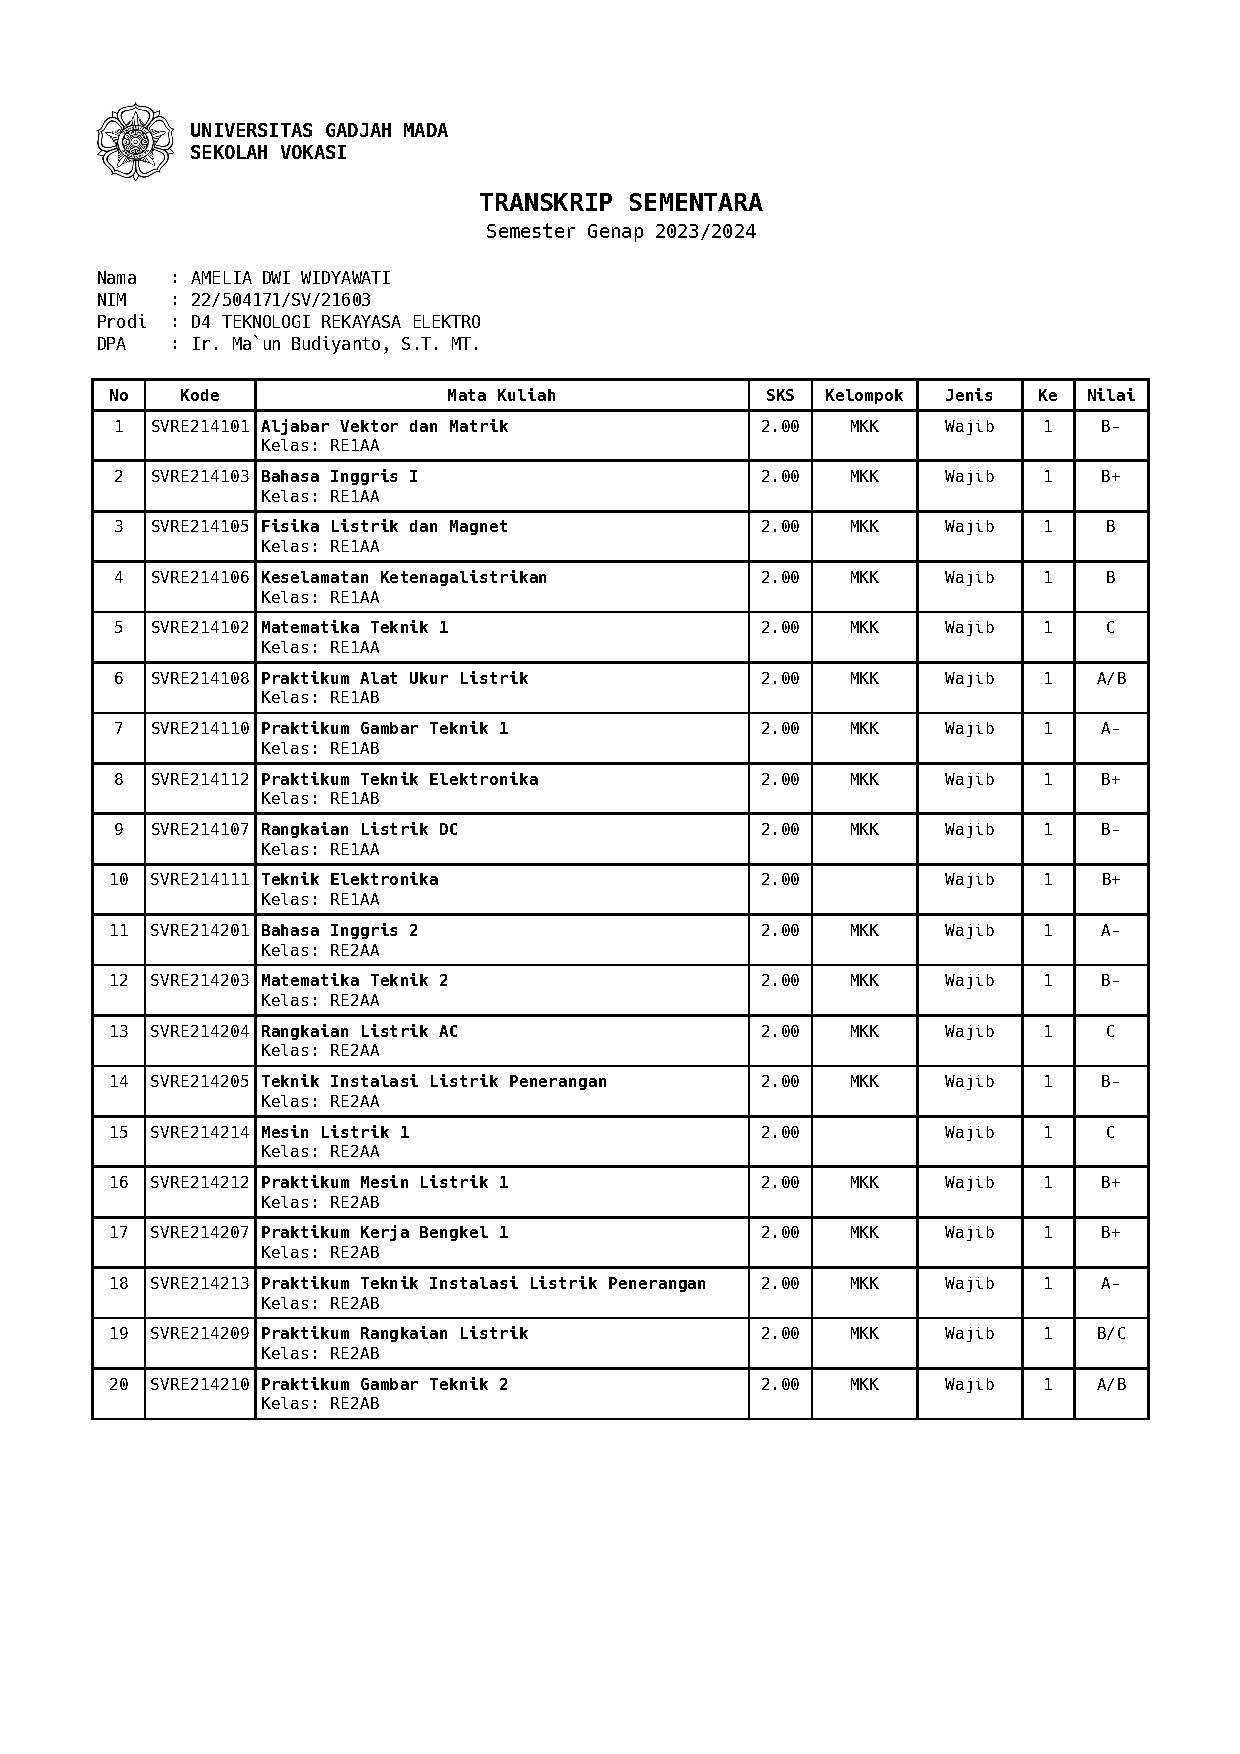
\includegraphics[scale=0.7,page=1]{dokumen/transkrip_amelia.pdf}
	\newpage
	\includegraphics[scale=0.7,page=2]{dokumen/transkrip_amelia.pdf}
	\newpage
	\includegraphics[scale=0.7,page=3]{dokumen/transkrip_amelia.pdf}
	\newpage
	\item Identitas Diri\\ [0.5cm]
	
\includegraphics[scale=0.7]{dokumen/identitas.jpg}
	
	
\end{itemize}



\section{Data Diri {\penulisKedua}}
\begin{itemize}
	
	
	
	\item Riwayat Diri\\
	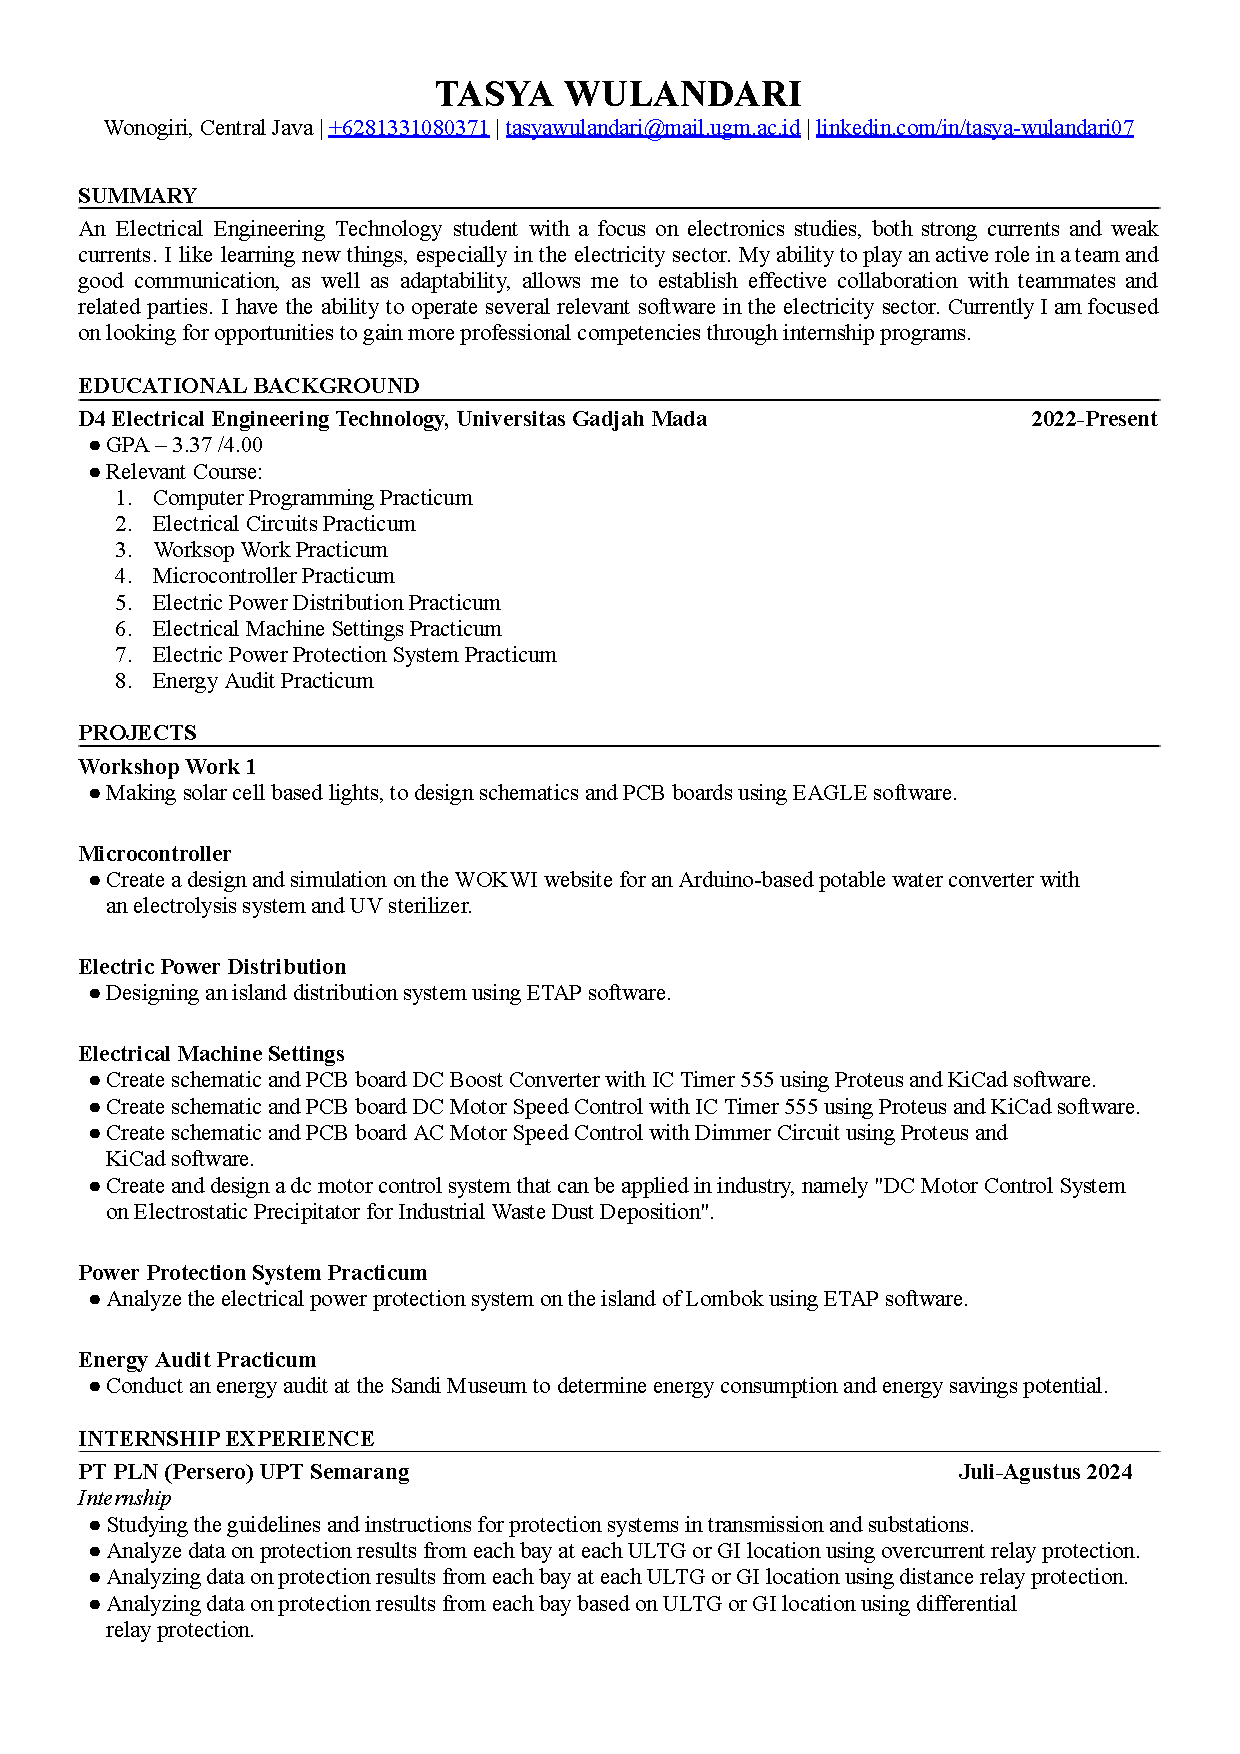
\includegraphics[scale=0.7,page=1]{dokumen/cv_tasya.pdf}
	\newpage
	\includegraphics[scale=0.7,page=2]{dokumen/cv_tasya.pdf}
	
	\newpage		
	\item Transkrip Nilai\\
	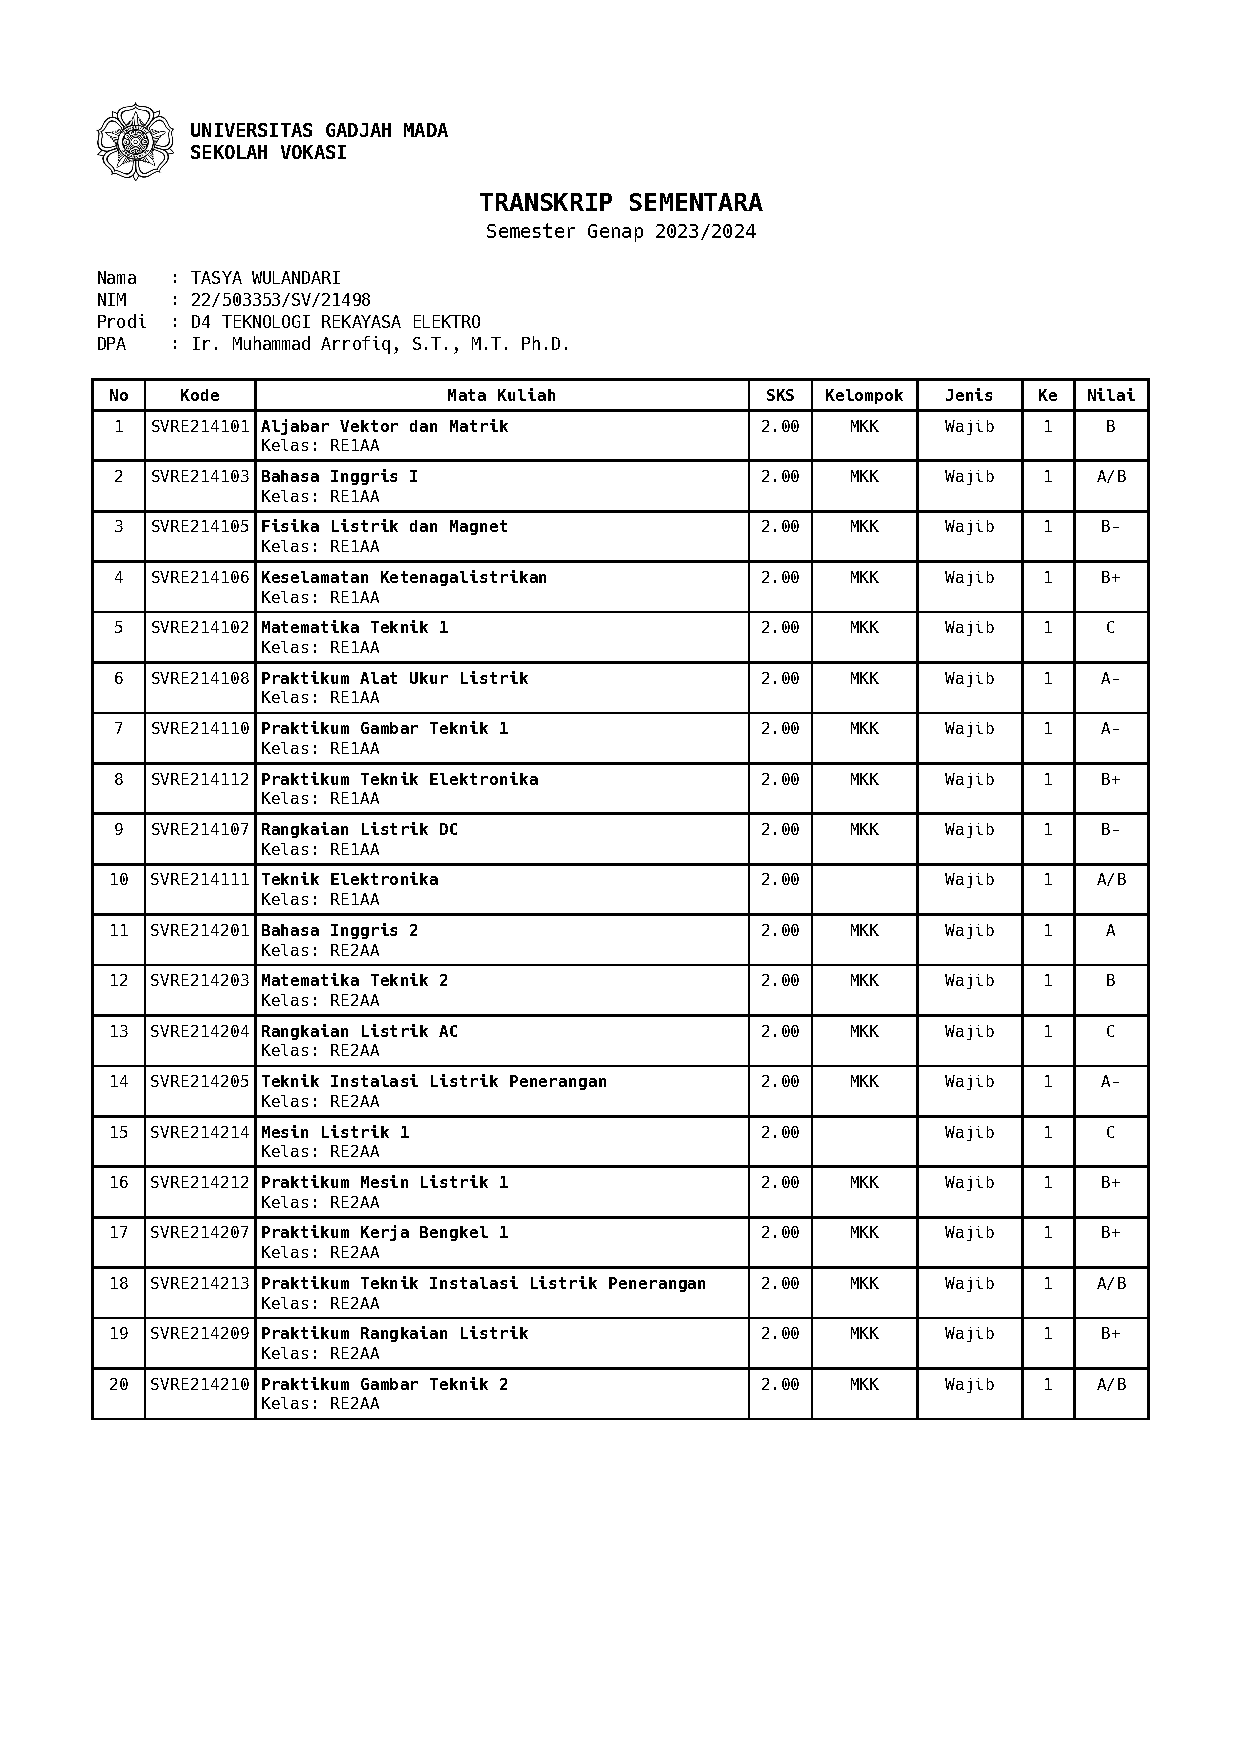
\includegraphics[scale=0.7,page=1]{dokumen/transkrip_tasya.pdf}
	\newpage
	\includegraphics[scale=0.7,page=2]{dokumen/transkrip_tasya.pdf}
	\newpage
	\includegraphics[scale=0.7,page=3]{dokumen/transkrip_tasya.pdf}
	\newpage
	\item Identitas Diri\\ [0.5cm]
	
\includegraphics[scale=0.7]{dokumen/identitas.jpg}
	
\end{itemize}
